\section{Annotated visualizations}
\label{sec:visuals}

The charts are produced by \file{scripts/figures\_analyse.py} from the CSV tables, without database access. Colors are consistent throughout: \textcolor{member}{\textbf{blue}} for members, \textcolor{casual}{\textbf{orange}} for casual riders. Each caption states the question asked, then the finding.

\begin{figure}[H]
\centering
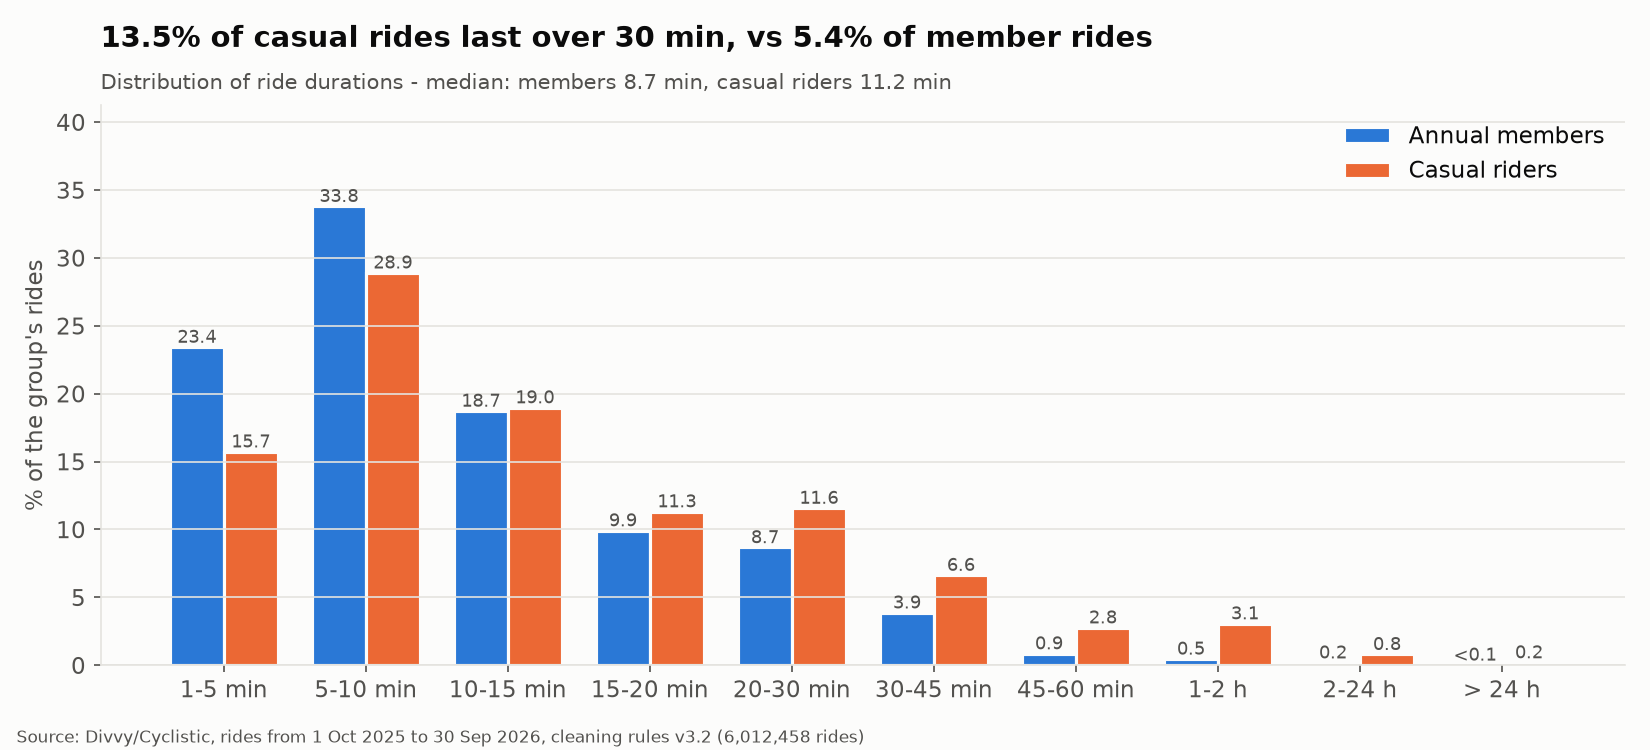
\includegraphics[width=0.94\linewidth]{f2_duration_distribution.png}
\caption{\textbf{Do both groups ride for as long?} No: rides of 1 to 10~min dominate among members (57.3\%), while casual riders are over-represented beyond 15~min; 13.5\% of their rides exceed 30~min, vs 5.4\%. \textit{(\file{f2\_duration\_distribution.png})}}
\label{fig:durations}
\end{figure}

\begin{figure}[H]
\centering
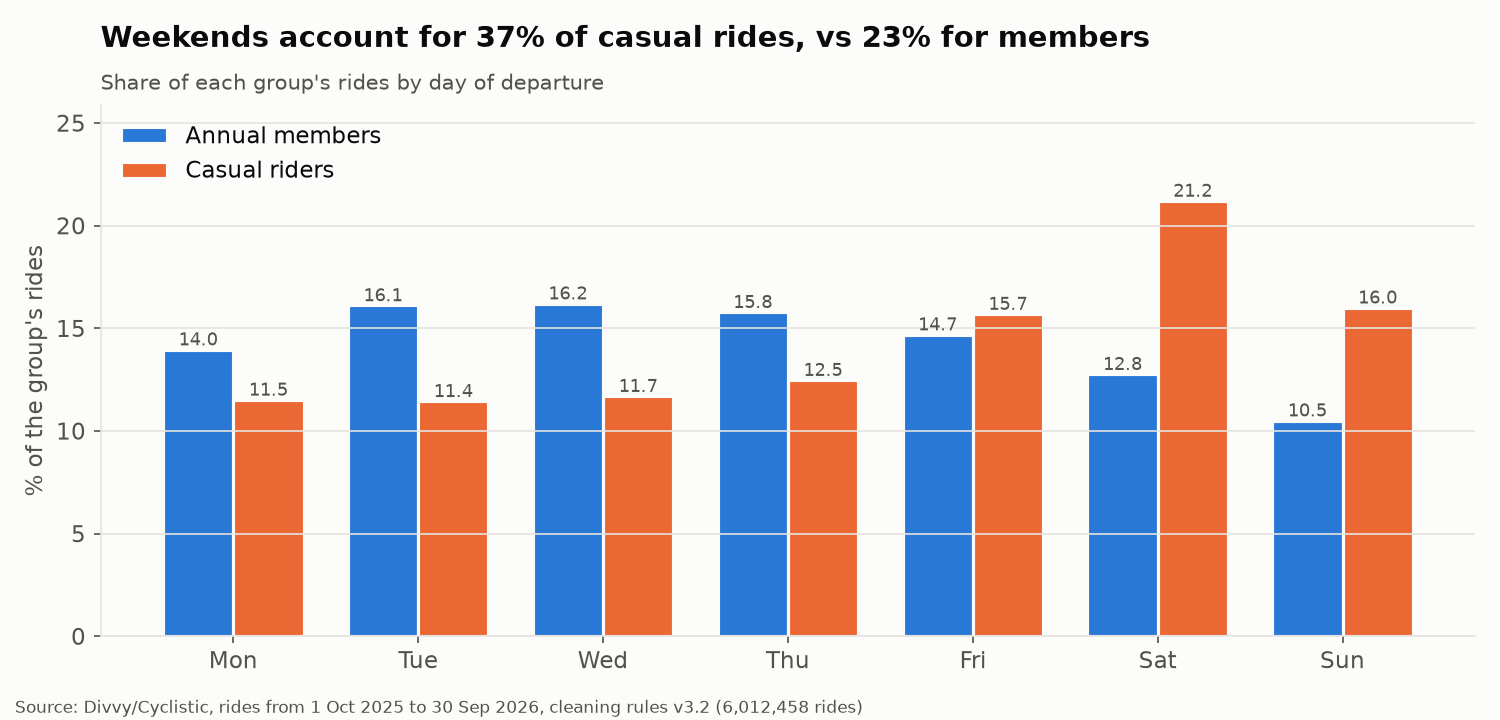
\includegraphics[width=0.94\linewidth]{f3_day_of_week.png}
\caption{\textbf{Do both groups ride on the same days?} Casual riders are over-represented at weekends (37.2\% of their rides vs 23.3\%), but most of their rides take place on weekdays. \textit{(\file{f3\_day\_of\_week.png})}}
\label{fig:days}
\end{figure}

\begin{figure}[H]
\centering
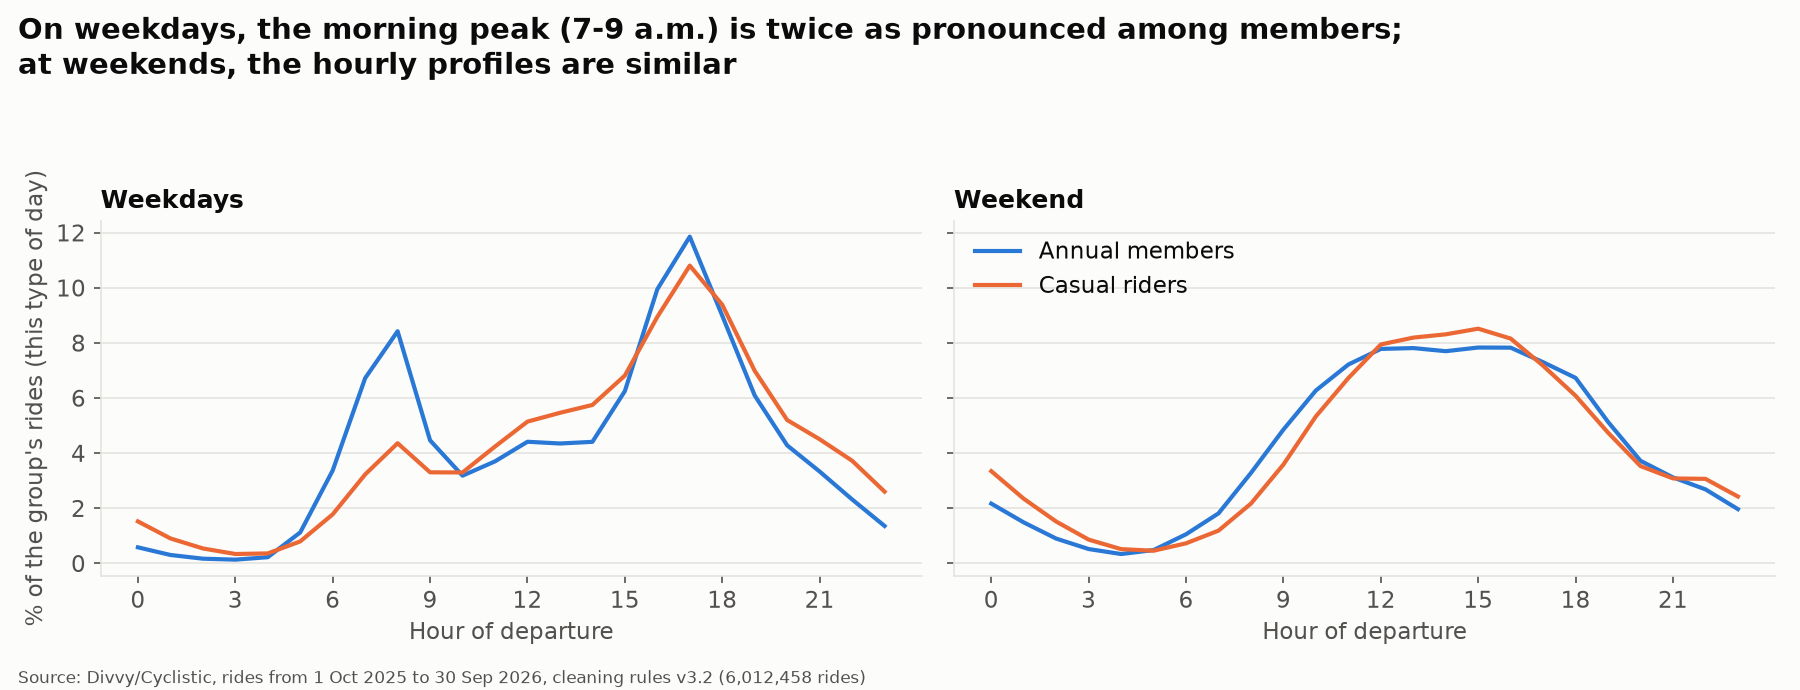
\includegraphics[width=0.98\linewidth]{f5_hourly_profile.png}
\caption{\textbf{At what time do they set off?} On weekdays, the morning peak (7--9 a.m.) is twice as pronounced among members; both groups peak at 5 p.m.; at weekends, the profiles are almost identical. \textit{(\file{f5\_hourly\_profile.png})}}
\label{fig:hours}
\end{figure}

\begin{figure}[H]
\centering
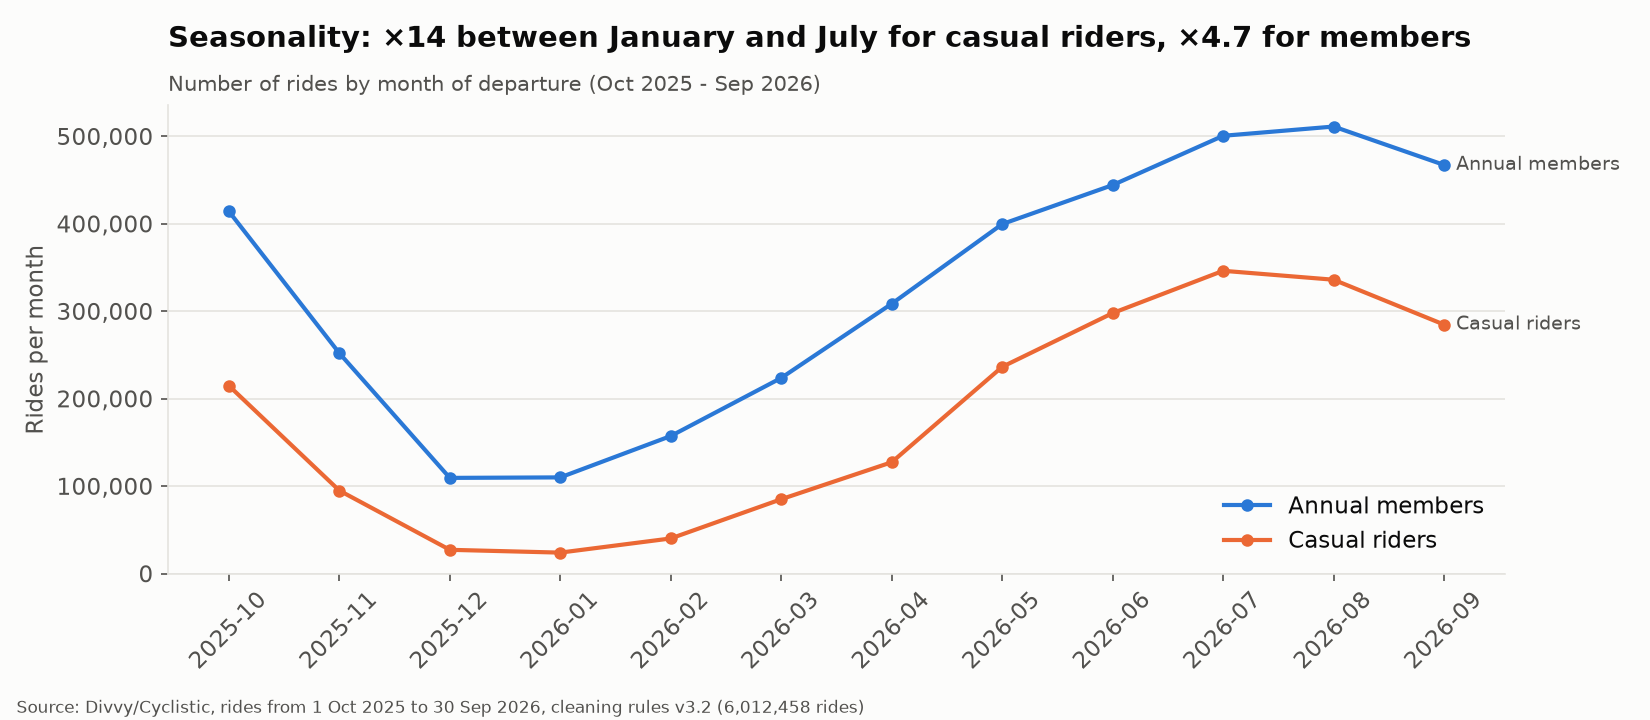
\includegraphics[width=0.94\linewidth]{f4_monthly_trend.png}
\caption{\textbf{Does usage vary with the season?} Same calendar, very different amplitude: ×14.4 between January and July for casual riders, ×4.7 between December and August for members. \textit{(\file{f4\_monthly\_trend.png})}}
\label{fig:months}
\end{figure}

\begin{figure}[H]
\centering
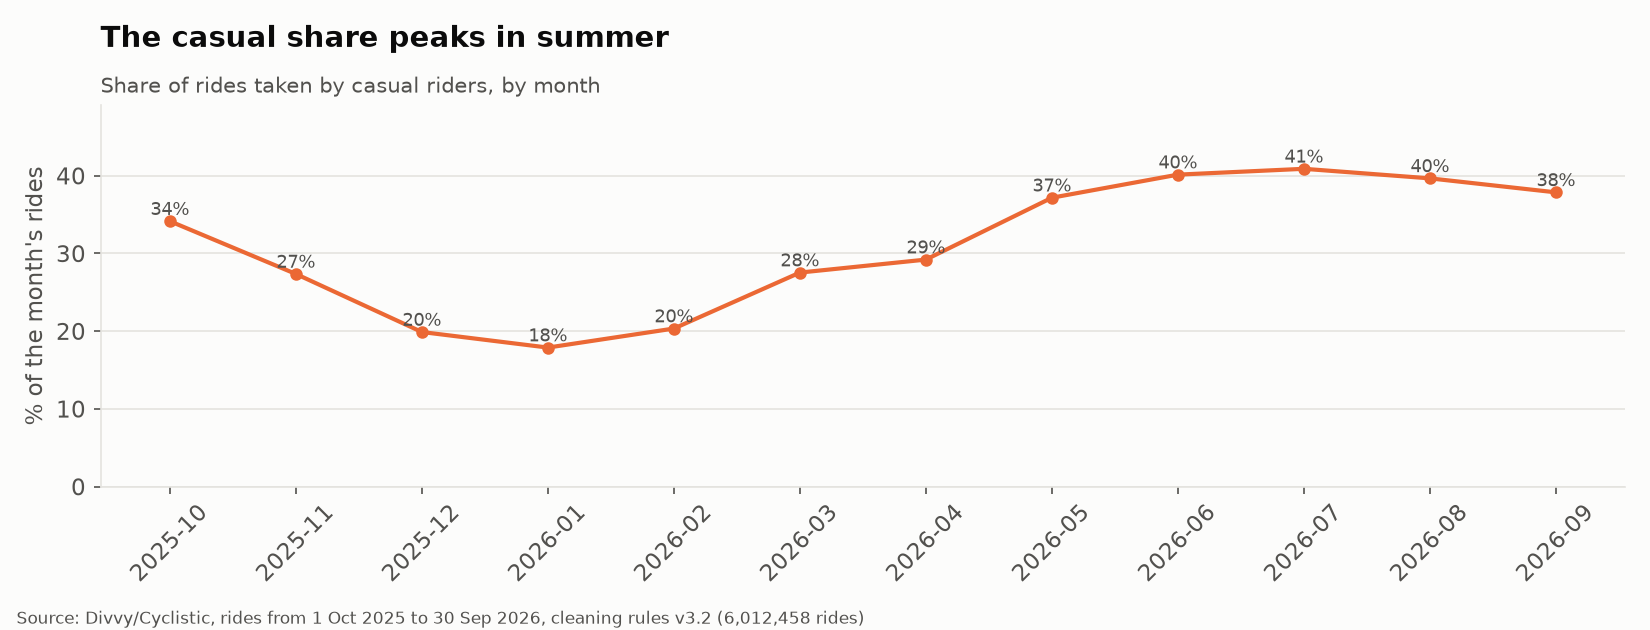
\includegraphics[width=0.94\linewidth]{f4b_casual_share_by_month.png}
\caption{\textbf{What share of activity do casual riders represent over the year?} From 17.9\% of rides in January to 40.9\% in July; more than 37\% from May to September. \textit{(\file{f4b\_casual\_share\_by\_month.png})}}
\label{fig:casualshare}
\end{figure}

\begin{figure}[H]
\centering
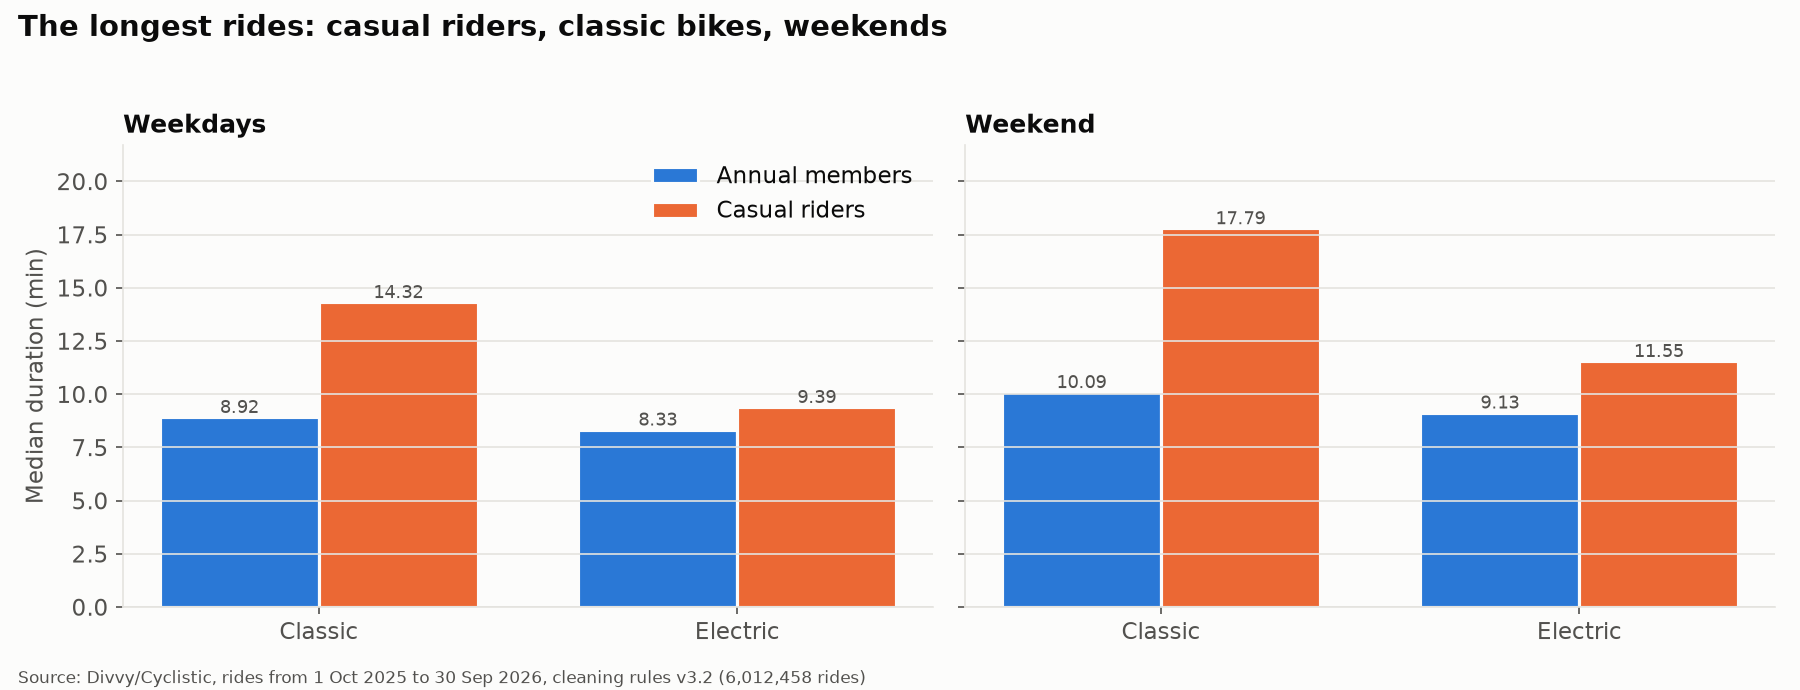
\includegraphics[width=0.98\linewidth]{f7_bike_type_by_day_type.png}
\caption{\textbf{Where is the duration gap largest?} On classic bikes at weekends (median 17.79 vs 10.09~min); on e-bikes on weekdays, the two groups are close (9.39 vs 8.33~min). \textit{(\file{f7\_bike\_type\_by\_day\_type.png})}}
\label{fig:bikes}
\end{figure}

\begin{figure}[H]
\centering
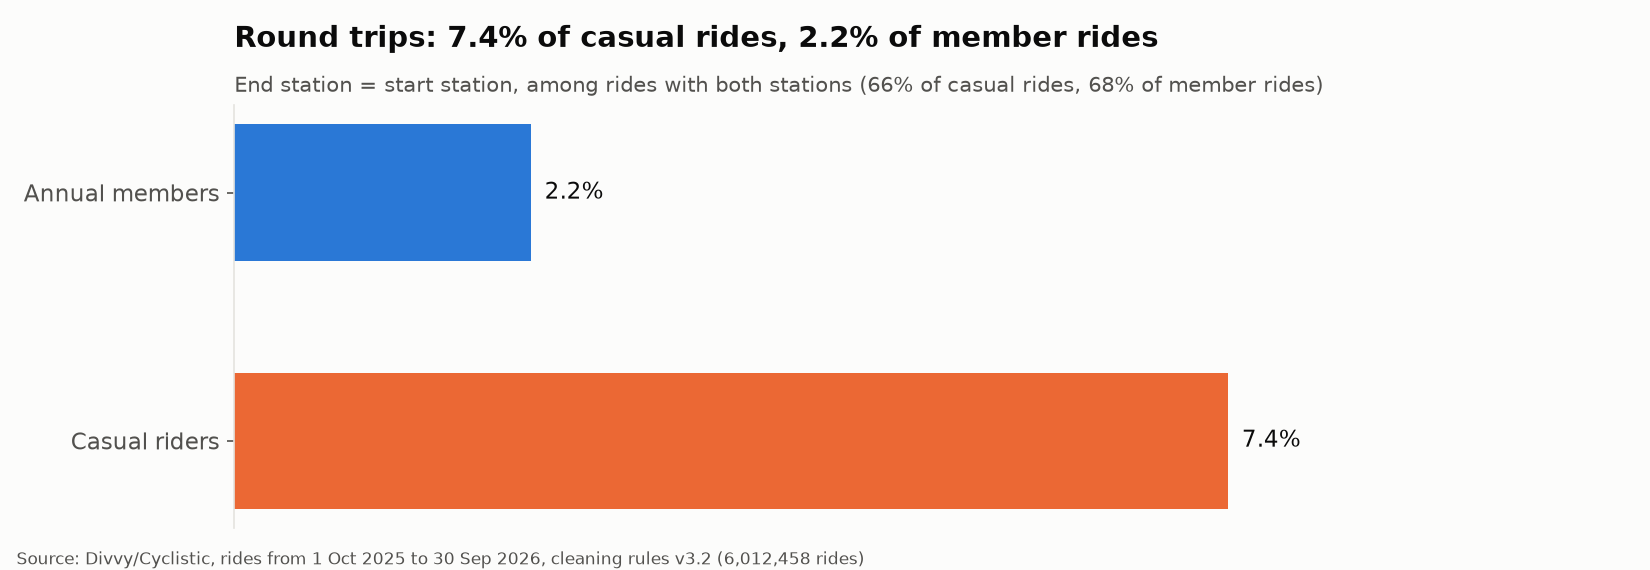
\includegraphics[width=0.86\linewidth]{f8_round_trips.png}
\caption{\textbf{Do rides return to their starting point?} 7.4\% of casual rides vs 2.2\% of member rides, among rides with both stations. \textit{(\file{f8\_round\_trips.png})}}
\label{fig:roundtrips}
\end{figure}
